\documentclass[10pt]{article}
\usepackage[polish]{babel}
\usepackage[utf8]{inputenc}
\usepackage[T1]{fontenc}
\usepackage{amsmath}
\usepackage{amsfonts}
\usepackage{amssymb}
\usepackage[version=4]{mhchem}
\usepackage{stmaryrd}
\usepackage{graphicx}
\usepackage[export]{adjustbox}
\graphicspath{ {./images/} }

\title{LIGA MATEMATYCZNA \\
 im. Zdzisława Matuskiego \\
 PAŹDZIERNIK 2022 \\
 SZKOŁA PODSTAWOWA \\
 klasy IV - VI }

\author{}
\date{}


\begin{document}
\maketitle
\section*{ZADANIE 1.}
W pewnym sześciokącie każde dwa kolejne boki są prostopadłe. Długości pięciu boków tego sześciokąta są równe 5, 6, 8, 10, 16. Jaką długość może mieć szósty bok?

\section*{ZADANIE 2.}
Prostokąt \(A B C D\) podzielono na trzy mniejsze prostokąty tak, jak na rysunku. Wyznacz pole środkowego prostokąta i jego wymiary wiedząc, że pola dwóch prostokątów i długości dwóch odcinków podane są na rysunku.\\
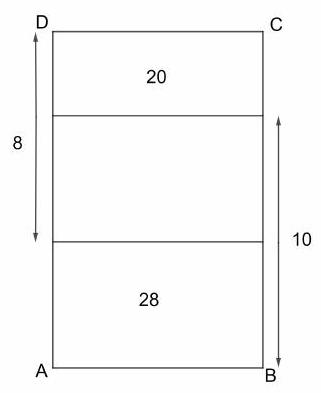
\includegraphics[max width=\textwidth, center]{2024_11_21_f6b427e3db4760b1cff2g-1}

\section*{ZADANIE 3.}
Ile jest liczb stucyfrowych, których iloczyn cyfr jest równy 6 ?

\section*{ZADANIE 4.}
Adam zbiera modele samochodów. W 11 ponumerowanych pudełkach ułożył 350 modeli. W każdych trzech kolejnych pudełkach liczba modeli jest równa 99. Ile modeli jest w szóstym pudełku?

\section*{ZADANIE 5.}
Ania i Bartek dostali od mamy 35 cukierków. Rozdzielili je na kilka talerzy, z których każdy zawierał więcej niż jeden cukierek. Następnie z każdego talerza zabrali po jednym cukierku i dołożyli je do pierwszego talerza. Wtedy okazało się, że na każdym talerzu jest tyle samo cukierków. Ile cukierków było początkowo na każdym talerzu?


\end{document}